\documentclass[10pt,letterpaper]{article}
\usepackage[latin1]{inputenc}
\usepackage{amsmath}
\usepackage{amsfonts}
\usepackage{amssymb}
\usepackage{makeidx}
\usepackage{graphicx}
\usepackage{algorithm2e}
\usepackage{float}
\usepackage[left=1.00in, right=1.00in, top=1.00in, bottom=1.00in]{geometry}
\author{Jay Ricco, David Van Chu}
\title{Introduction to Artificial Intelligence\\Analysis of Boundary Trees and Differentiable Boundary Trees}
\begin{document}
	\maketitle
	\section{Motivation}
	The goal of this project was to understand, evaluate, and further study the properties of the Boundary Tree$^1$ and Differentiable Boundary Tree$^2$ algorithms, presented in their respective papers, The Boundary Forest Algorithm for Online Supervised and Unsupervised Learning, and Learning Deep Nearest Neighbor Representations Using Differentiable Boundary Trees.
	\section{Boundary Trees}
		\hspace{5mm}Features are the attributes of an input, or example. With the MNIST data set, each example is composed of 784 pixels, each one of which are considered the features.
		
		\vspace{2mm}
		The goal for Boundary Trees was to create a learning algorithm that is quick to train, quick to query, on-line and instance-based. On-line means that it's able to consistently accept and train new examples as it's running.
		
		\vspace{2mm}
		To query the Boundary Tree, we take an example as an input and find the closest node using Euclidean distance as the distance function. We return the closest node, and from that, we can get the class associated with the node. This is the class that the Boundary Tree thinks the example is.
		
		\vspace{2mm}
		To train the Boundary Tree, we query the existing tree with the example, and if the node returned does not have the same class as the example's target class, we add a new node to the tree with the example and corresponding target class.

	\section{Observations (MNIST)}
		Initial observations indicated that:
		\begin{enumerate}
			\item The maximum branching factor value (k) is crucial with respect to the performance of the algorithm on a given data set.
			\item While the total testing time and accuracy plateau, with $\uparrow$ examples, training time $\epsilon O(n).$
			\item BT's perform far better with MNIST than CIFAR; this shows inadequacy of the Euclidean distance metric for high feature complexity use-cases.
		\end{enumerate}
		
		After running the tests, we noticed that setting the branching factor to 5-10 seemed to be the best if both time and accuracy is a concern, as anything less than 5 will result in lower accuracy while taking about the same amount of time to train and test. With branching factors larger than 10, training and testing time grew quite a bit with only a small increase in accuracy.
		
		Another interesting point is that with a larger branching factor, the training time itself varies by quite a bit, ranging from 140.47 seconds to 223.79 seconds, whereas tests ran with a lower branching factor resulted in consistent training times.
		
		\begin{figure}[H]
			\caption{For each test the branching factor is changed, and each data point was acquired by taking an average over 10 runs.}
			\centering
			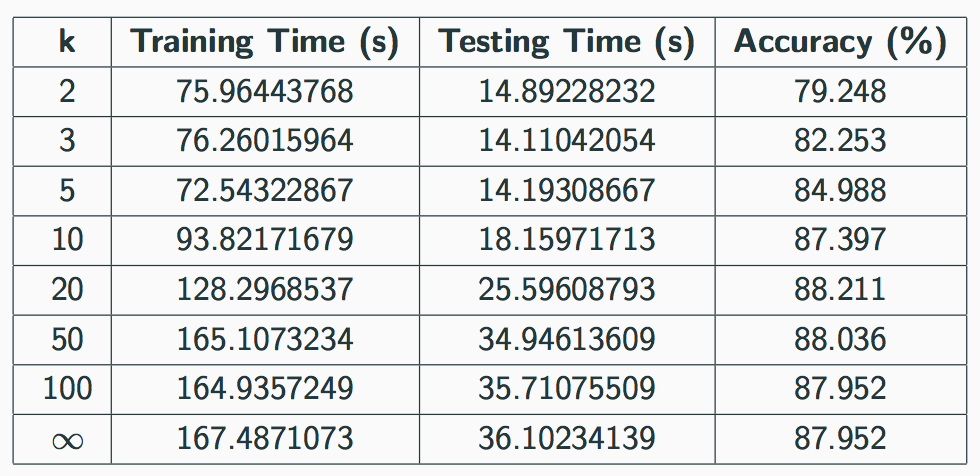
\includegraphics[width=0.60\textwidth]{mnist_varying_k.png}
		\end{figure}
	
		\begin{figure}[H]
			\caption{MNIST dataset, varying the number of examples, averaged over 10 runs.}
			\centering
			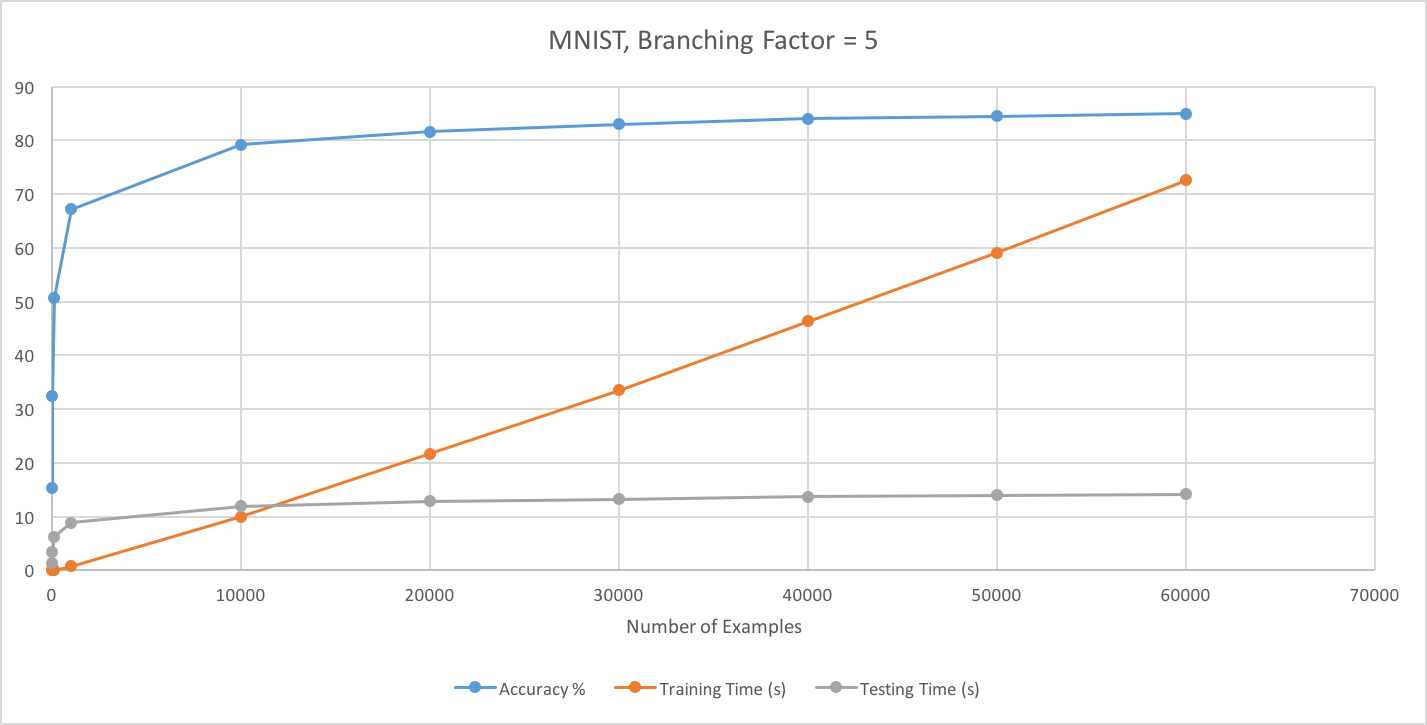
\includegraphics[width=0.60\textwidth]{mnistk5.png}
			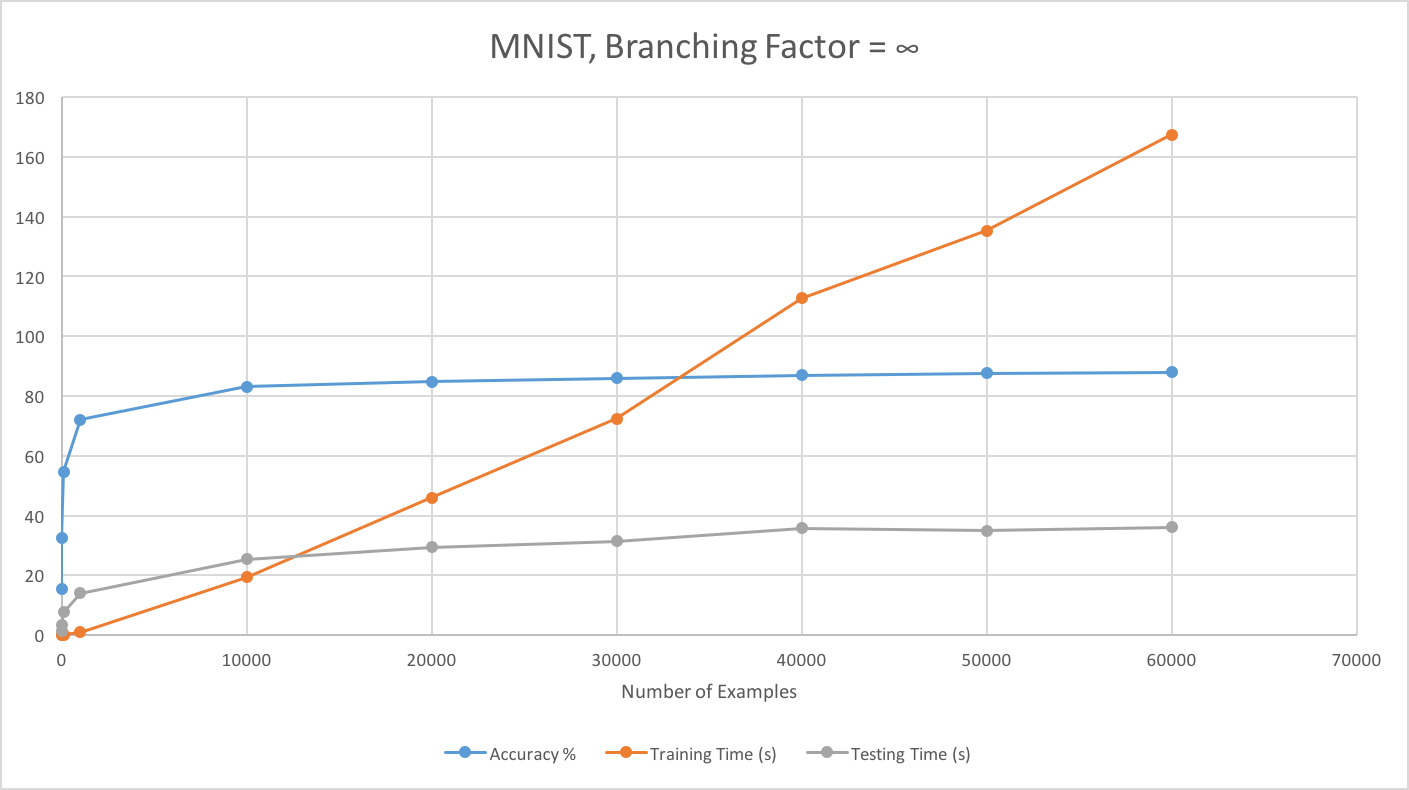
\includegraphics[width=0.60\textwidth]{mnistkinfinity.png}
		\end{figure}
		
		
		\section{Observations (CIFAR10)}
		\hspace{5mm}We see similar results when using Boundary Trees on the CIFAR10 dataset, although it never achieves over 27.7$\%$ accuracy. Using a smaller branching factor quickens the training time significantly compared to the MNIST dataset results.
		
		\begin{figure}[H]
			\caption{For each test the branching factor is changed, and each data point was acquired by taking an average over 10 runs.}
			\centering
			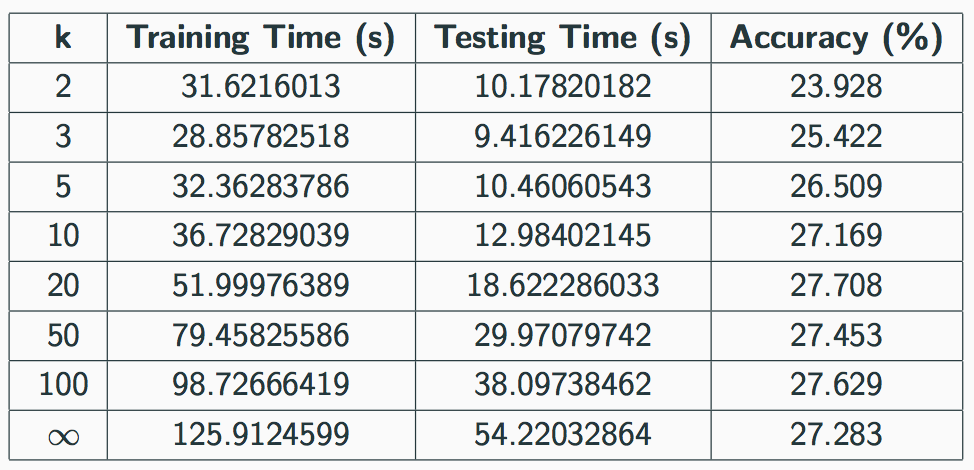
\includegraphics[width=0.60\textwidth]{cifar10_varying_k.png}
		\end{figure}
		
		\begin{figure}[H]
		\caption{CIFAR10 dataset, varying the number of examples, averaged over 10 runs.}
		\centering
		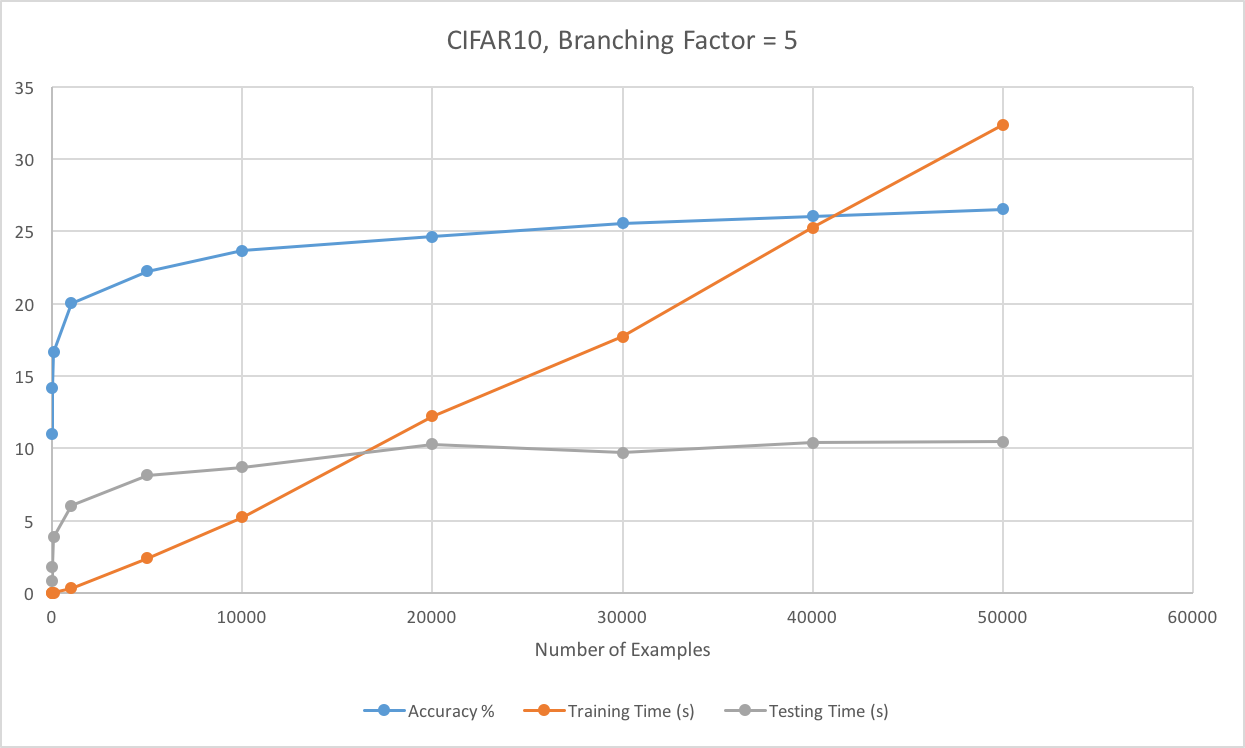
\includegraphics[width=0.60\textwidth]{cifar10k5.png}
		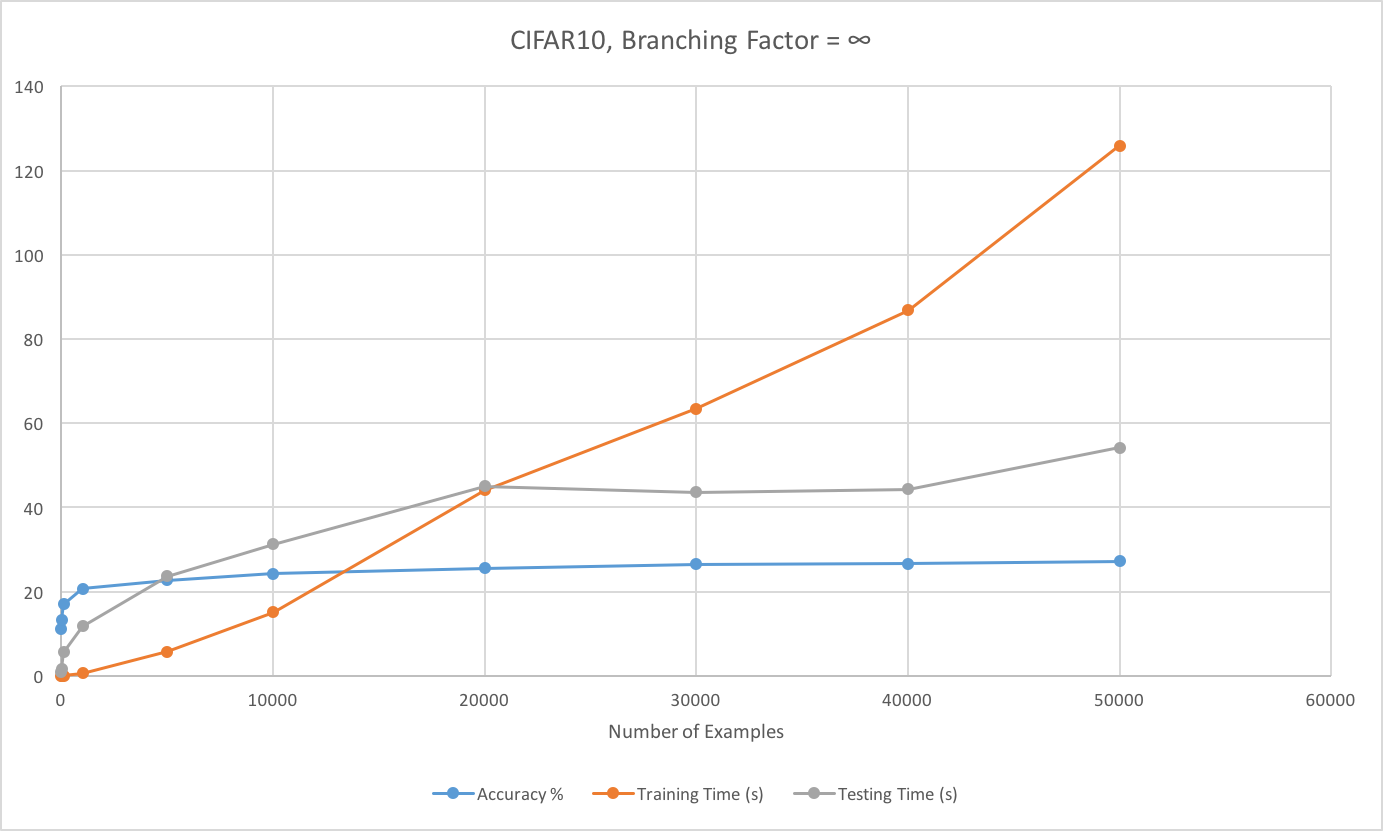
\includegraphics[width=0.60\textwidth]{cifar10kinfinity.png}
		\end{figure}
		
\end{document}